\section{Operations on Sets}
        Similar to the arithmetic of real numbers, there
        are standard operations that can be performed on
        sets to obtain new sets. The four most common
        operations are union, intersection, set difference,
        and symmetric difference. Often the
        \textit{complement} of a set is discussed, but as
        we will see, this is just a specific case of set
        difference.
        \begin{figure}[H]
            \centering
            %--------------------------------Dependencies----------------------------------%
%   tikz                                                                       %
%-------------------------------Main Document----------------------------------%
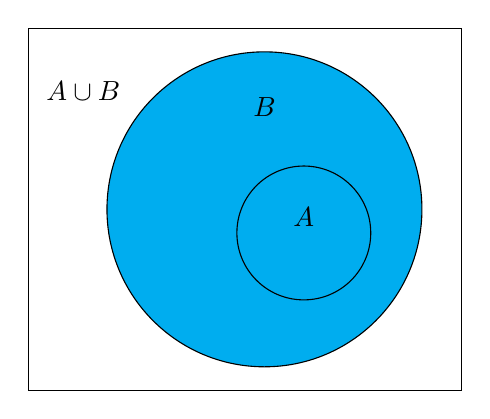
\begin{tikzpicture}
    \draw (-3,-2.3) rectangle (2.5,2.3);
    \draw[fill=cyan] (0,0) circle (2);
    \draw (0.5,-0.3) circle (0.85);

    \node at (0.5,-0.1) {$A$};
    \node at (0,1.3) {$B$};
    \node at (-2.3,1.5) {$A\cup{B}$};
\end{tikzpicture}
            \caption{Visual for Thm.~\ref{thm:Union_With_Subset}.}
            \label{fig:Venn_Diagram_Union_With_Subset}
        \end{figure}
        Set operations are very algebraic, and it is often
        useful to build up several small tools to eventually
        prove larger theorems in a simple way. We wish to
        show that union is commutative and associative, and
        that there is an \textit{identity}.
        \begin{ltheorem}{Commutative Law of Unions}{Commutative_Law_of_Unions}
            If $A$ and $B$ are sets, then $A\cup{B}=B\cup{A}$.
        \end{ltheorem}
        \begin{proof}
            For if $x\in{A}\cup{B}$, then either $x\in{A}$ or $x\in{B}$, or
            both (Def.~\ref{def:Union_of_Two}). But then either $x\in{B}$ or
            $x\in{A}$, or both, and therefore $x\in{B}\cup{A}$
            (Def.~\ref{def:Union_of_Two}). But then for all $x\in{A}\cup{B}$
            it is true that $x\in{B}\cup{A}$, and therefore
            $A\cup{B}\subseteq{B}\cup{A}$ (Def.~\ref{def:Subsets}). Similarly,
            $B\cup{A}\subseteq{A}\cup{B}$, and thus $A\cup{B}=B\cup{A}$
            (Def.~\ref{def:Equal_Sets}). Therefore, etc.
        \end{proof}
        When taking the union of two sets, we obtain a
        \textit{larger} set, in a sense. Again relying on
        the analogy of arithmetic, given two non-negative
        integers $a$ and $b$, it is true that $a\leq{a}+b$.
        Equality is obtained if and only if either $a$ or
        $b$ is equal to zero. As we will see, the empty set
        acts as the \textit{zero} of unions. Also, given
        three non-negative integers $a$, $b$, and $c$, if
        $b\leq{c}$, then $a+b\leq{a}+c$. A similar result
        will hold for sets and unions.
        \begin{theorem}
            \label{thm:Union_is_Bigger}%
            If $A$ and $B$ are sets, then
            $A\subseteq{A}\cup{B}$.
        \end{theorem}
        \begin{proof}
            For suppose not. Then there is an $x\in{A}$ such
            that $x\notin{A}\cup{B}$. But if $x\in{A}$, then
            $x\in{A}$ or $x\in{B}$ and thus $x\in{A}\cup{B}$
            (Def.~\ref{def:Union_of_Two}), a
            contradiction. Therefore, etc.
        \end{proof}
        \begin{theorem}
            \label{thm:Union_With_Lesser_Set}%
            If $A$, $B$, and $C$ are sets, and if
            $B\subseteq{C}$, then
            $A\cup{B}\subseteq{A}\cup{C}$.
        \end{theorem}
        \begin{proof}
            For if $x\in{A}\cup{B}$, then either $x\in{A}$,
            or $x\in{B}$, or both
            (Def.~\ref{def:Union_of_Two}). But $B$ is a
            subset of $C$, and therefore if $x\in{B}$, then
            $x\in{C}$ (Def.~\ref{def:Subsets}).
            Thus, if $x\in{A}$ or $x\in{B}$, then
            $x\in{A}$ or $x\in{C}$, and therefore
            $x\in{A}\cup{C}$ (Def.~\ref{def:Union_of_Two}).
            Thus, $A\cup{B}\subseteq{A}\cup{C}$
            (Def.~\ref{def:Subsets}). Therefore, etc.
        \end{proof}
        \begin{theorem}
            If $A$, $B$, $C$, and $D$ are sets, if
            $A\subseteq{C}$, and if $B\subseteq{D}$, then
            $A\cup{B}\subseteq{C}\cup{D}$.
        \end{theorem}
        \begin{proof}
            For if $B\subseteq{D}$, then
            $A\cup{B}\subseteq{A}\cup{D}$
            (Thm.~\ref{thm:Union_With_Lesser_Set}).
            But $A\cup{D}=D\cup{A}$
            (Thm.~\ref{thm:Commutative_Law_of_Unions}).
            But if $A\subseteq{C}$, then
            $D\cup{A}\subseteq{D}\cup{C}$
            (Thm.~\ref{thm:Union_With_Lesser_Set}). But
            $D\cup{C}=C\cup{D}$
            (Thm.~\ref{thm:Commutative_Law_of_Unions}).
            And if $A\cup{B}\subseteq{A}\cup{D}$ and
            $A\cup{D}\subseteq{C}\cup{D}$, then
            $A\cup{B}\subseteq{C}\cup{D}$
            (Thm.~\ref{thm:Subset_is_Transitive}).
            Therefore, etc.
        \end{proof}
        Taking the union of subsets is redundant, as we
        simply obtain the larger set. This starts to break
        down the analogy between sets and arithmetic, since
        there is only one \textit{zero}. That is, there is
        only one number $b$ such that $a+b=a$, and that is
        $b=0$. While any subset acts as a \textit{zero} of a
        given set, the empty set has the property that it
        acts as a zero for \textit{every} set. It is the only
        set with this property, and thus the analogy with
        arithmetic is restored.
        \begin{theorem}
            \label{thm:Union_With_Subset}%
            If $A$ and $B$ are sets, and if
            $A\subseteq{B}$, then $A\cup{B}=B$.
        \end{theorem}
        \begin{proof}
            For if $A$ and $B$ are sets, then
            $B\subseteq{A}\cup{B}$
            (Thm.~\ref{thm:Union_is_Bigger}).
            But if $A\subseteq{B}$, then for all $x\in{A}$,
            it is true that $x\in{B}$
            (Def.~\ref{def:Subsets}). Thus if $x\in{A}$ or if
            $x\in{B}$, then $x\in{B}$. But then, for all
            $x\in{A}\cup{B}$, it is true that $x\in{B}$, and
            therefore $A\cup{B}\subseteq{B}$
            (Def.~\ref{def:Subsets}). Thus,
            $A\cup{B}=B$ (Def.~\ref{def:Equal_Sets}).
            Therefore, etc.
        \end{proof}
        \begin{theorem}
            \label{thm:Union_with_Emptyset}%
            If $A$ is a set, then $A=\emptyset\cup{A}$.
        \end{theorem}
        \begin{proof}
            For $\emptyset\subseteq{A}$
            (Thm.~\ref{thm:Emptyset_Is_Subset}) and
            therefore $\emptyset\cup{A}=A$
            (Thm.~\ref{thm:Union_With_Subset}).
        \end{proof}
        \begin{theorem}
            \label{thm:Empty_Set_Is_Zero_for_Unions}%
            If $A$ is a set such that, for any set $B$, it is
            true that $A\cup{B}=B$, then $A$ is the
            empty set.
        \end{theorem}
        \begin{proof}
            For suppose not. If $A\ne\emptyset$, then there
            is an $x\in{A}$ (Def.~\ref{def:Empty_Set}).
            But then $B=\{A\}$ is a set
            (Def.~\ref{def:Sets}). But then $x\in{A}\cup{B}$
            (Def.~\ref{def:Union_of_Two}). But $x\notin{B}$,
            and thus $A\cup{B}\ne{B}$
            (Def.~\ref{def:Equal_Sets}), a contradiction
            since $A$ is such that for any set $B$, it is
            true that $A\cup{B}=B$. Therefore, etc.
        \end{proof}
        Thm.~\ref{thm:Empty_Set_Is_Zero_for_Unions} proves
        the assertion that the empty set is the zero of set
        union. The converse of
        Thm.~\ref{thm:Union_With_Subset} can be proved as
        well.
        \begin{theorem}
            \label{thm:Conv_Union_Is_Bigger}%
            If $A$ and $B$ are sets, and if
            $A\cup{B}\subseteq{A}$, then $A\cup{B}=A$.
        \end{theorem}
        \begin{proof}
            For $A\subseteq{A}\cup{B}$
            (Thm.~\ref{thm:Union_is_Bigger}). But by
            hypothesis, $A\cup{B}\subseteq{A}$. But then
            $A=A\cup{B}$ (Def.~\ref{def:Equal_Sets}).
            Therefore, etc.
        \end{proof}
        \begin{theorem}
            \label{thm:Union_is_Equal}%
            If $A$ and $B$ are sets, and if
            $A\cup{B}\subseteq{A}$, then $B\subseteq{A}$.
        \end{theorem}
        \begin{proof}
            For if $A\cup{B}\subseteq{A}$, then
            $A\cup{B}=A$
            (Thm.~\ref{thm:Conv_Union_Is_Bigger}). And also,
            $B\subseteq{A}\cup{B}$
            (Thm.~\ref{thm:Union_is_Bigger}). But if
            $A\cup{B}=A$ and $B\subseteq{A}\cup{B}$, then
            $B\subseteq{A}$
            (Thm.~\ref{thm:Subsets_of_Equal_Sets}).
            Therefore, etc.
        \end{proof}
        We'll wrap up unions by showing that the operation
        is associative. Once again relying on the analogy
        of arithmetic, given three real numbers $a$, $b$,
        and $c$, it is true that $a+(b+c)=(a+b)+c$. This
        is called the associative law of addition. Combining
        this law with the commutative law shows that the
        order in which three real numbers are added is
        irrelevant. Applying induction, we see that given
        any finite collection of real numbers, the order in
        which we add them is again irrelevant. The same holds
        true for the union of sets.
        \begin{theorem}
            \label{thm:First_Assoc_Law_Union}%
            If $A$, $B$, and $C$ are sets, then
            $A\cup(B\cup{C})\subseteq(A\cup{B})\cup{C}$.
        \end{theorem}
        \begin{proof}
            For $B\subseteq{A}\cup{B}$
            (Thm.~\ref{thm:Union_is_Bigger}), and thus
            $B\cup{C}\subseteq(A\cup{B})\cup{C}$
            (Thm.~\ref{thm:Union_With_Lesser_Set}). But then
            $A\cup(B\cup{C})\subseteq{A}%
             \cup((A\cup{B})\cup{C})$
            (Thm.~\ref{thm:Union_With_Lesser_Set}).
            But $A\subseteq{A}\cup{B}$ and
            $A\cup{B}\subseteq(A\cup{B})\cup{C}$
            (Thm.~\ref{thm:Union_is_Bigger}), and therefore
            $A\subseteq(A\cup{B})\cup{C}$
            (Thm.~\ref{thm:Subset_is_Transitive}). But then
            $(A\cup)B\cup{C}={A}\cup((A\cup{B})\cup{C})$
            (Thm.~\ref{thm:Union_With_Subset}). But it was
            proved that
            $A\cup(B\cup{C})\subseteq{A}%
             \cup((A\cup{B})\cup{C})$, and therefore
            $A\cup(B\cup{C})\subseteq(A\cup{B})\cup{C}$
            (Thm.~\ref{thm:Subsets_of_Equal_Sets}).
            Therefore, etc.
        \end{proof}
        \begin{ltheorem}{Associative Law of Unions}
              {Associative_Law_of_Unions}
            If $A$, $B$, and $C$ are sets, then
            $A\cup(B\cup{C})=(A\cup{B})\cup{C}$.
        \end{ltheorem}
        \begin{proof}
            For by the Commutative Law of Unions
            (Thm.~\ref{thm:Commutative_Law_of_Unions}),
            we have:
            \begin{equation}
                (A\cup{B})\cup{C}=C\cup(A\cup{B})
                                 =C\cup(B\cup{A})
            \end{equation}
            But $C\cup(B\cup{A})\subseteq(C\cup{B})\cup{A}$
            (Thm.~\ref{thm:First_Assoc_Law_Union}). Again by
            commutativity, we obtain:
            \begin{equation}
                (C\cup{B})\cup{A}=A\cup(C\cup{B})
                                 =A\cup(B\cup{C})
            \end{equation}
            Therefore,
            $(A\cup{B})\cup{C}\subseteq{A}\cup(B\cup{C})$.
            But $A\cup(B\cup{C})\subseteq(A\cup{B})\cup{C}$
            (Thm.~\ref{thm:First_Assoc_Law_Union}),
            and thus $A\cup(B\cup{C})=(A\cup{B})\cup{C}$
            (Def.~\ref{def:Equal_Sets}). Therefore, etc.
        \end{proof}
        \begin{theorem}
            \label{thm:Redundant_Union}%
            If $A$, $B$, and $C$ are sets and if
            $A\subseteq{B}$, then
            $A\cup(B\cup{C})=B\cup{C}$
        \end{theorem}
        \begin{proof}
            For $B\cup{C}\subseteq{A}\cup(B\cup{C})$
            (Thm.~\ref{thm:Union_is_Bigger}). But
            $A\cup(B\cup{C})=(A\cup{B})\cup{C}$
            (Thm.~\ref{thm:Associative_Law_of_Unions}).
            And since $A$ is a subset of $B$,
            $A\cup{B}=B$ (Thm.~\ref{thm:Union_With_Subset}),
            and thus $(A\cup{B})\cup{C}=B\cup{C}$. Thus,
            $B\cup{C}=A\cup(B\cup{C})$
            (Thm.~\ref{thm:Equality_Transitive}).
            Therefore, etc.
        \end{proof}
        \begin{ldefinition}{Intersection of Two Sets}
              {Intersection_of_Two}
            The intersection of two sets $A$ and $B$,
            denoted $A\cap{B}$, is the set:
            \begin{equation}
                A\cap{B}
                =\{\;x\,:\,x\in{A}\textrm{ and }x\in{B}\;\}
            \end{equation}
            That is, the set of elements $x$ that are in
            both $A$ and $B$.
        \end{ldefinition}
        Similar to set union, intersections can be visualized
        by Venn diagrams. See
        Fig.~\ref{fig:Union_Intersection_venn_diagram}.
        \begin{figure}[H]
            \centering
            \captionsetup{type=figure}
            \documentclass[crop,class=article]{standalone}
%----------------------------Preamble-------------------------------%
\usepackage{tikz}                       % Drawing/graphing tools.
%--------------------------Main Document----------------------------%
\begin{document}
    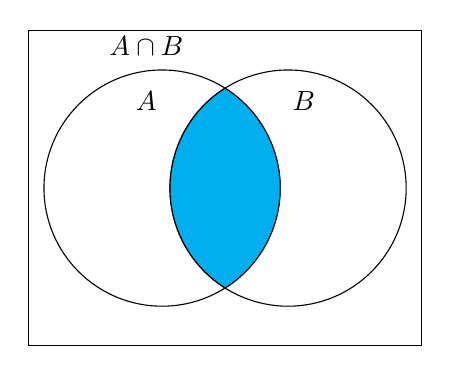
\begin{tikzpicture}
        \draw (-2.5,-2) rectangle (2.5,2);
        \draw (-0.8cm,0) circle (1.5cm);
        \draw (0.8cm,0) circle (1.5cm);
        \draw[fill=cyan]
            (0,-1.26886) arc(-57.77:57.77:1.5)
                         arc(122.231:237.7690:1.5);
        \node at (-1,1.1) {$A$};
        \node at (1,1.1) {$B$};
        \node at (-1,1.8) {$A\cap{B}$};
    \end{tikzpicture}
\end{document}
            \caption{Venn Diagrams for Intersections}
            \label{fig:Union_Intersection_venn_diagram}
        \end{figure}
        \begin{ltheorem}{Commutative Law of Intersections}
                        {Commut_Law_Intersec}
            If $A$ and $B$ are sets, then $A\cap{B}=B\cap{A}$.
        \end{ltheorem}
        \begin{proof}
            For if $x\in{A}\cap{B}$, then $x\in{A}$ and
            $x\in{B}$. But then $x\in{B}$ and $x\in{A}$,
            and therefore $x\in{B}\cap{A}$
            (Def.~\ref{def:Intersection_of_Two}). But then
            for all $x\in{A}\cap{B}$ it is true that
            $x\in{B}\cap{A}$, and therefore
            $A\cup{B}\subseteq{B}\cup{A}$
            (Def.~\ref{def:Subsets}). Similarly,
            $B\cap{A}\subseteq{A}\cap{B}$, and thus
            $A\cap{B}=B\cap{A}$ (Def.~\ref{def:Equal_Sets}).
            Therefore, etc.
        \end{proof}
        \begin{theorem}
            \label{thm:Intersection_is_Smaller}%
            If $A$ snd $B$ are sets, then
            $A\cap{B}\subseteq{A}$.
        \end{theorem}
        \begin{proof}
            If $x\in{A}\cap{B}$, then $x\in{A}$ and
            $x\in{B}$, and thus $x\in{A}$. Therefore, etc.
        \end{proof}
        \begin{theorem}
            \label{thm:Intersection_with_Lesser_Set}%
            If $A$, $B$, and $C$ are sets, and if
            $B\subseteq{C}$, then
            $A\cap{B}\subseteq{A}\cap{C}$.
        \end{theorem}
        \begin{proof}
            For if $x\in{A}\cap{B}$, then $x\in{A}$ and
            $x\in{B}$ (Def.~\ref{def:Intersection_of_Two}).
            But $B$ is a subset of $C$, and thus if
            $x\in{B}$, then $x\in{C}$
            (Def.~\ref{def:Subsets}). But then $x\in{A}$ and
            $x\in{C}$, and therefore $x\in{A}\cap{C}$
            (Def.~\ref{def:Intersection_of_Two}). But
            then $A\cap{B}\subseteq{A}\cap{C}$
            (Def.~\ref{def:Subsets}). Therefore, etc.
        \end{proof}
        \begin{theorem}
            \label{thm:Intersection_is_Equal}%
            If $A$ and $B$ are sets, and if
            $A=A\cap{B}$, then $A\subseteq{B}$.
        \end{theorem}
        \begin{proof}
            For suppose not. Then there is an $x\in{A}$ such
            that $x\notin{B}$. But since $A=A\cap{B}$,
            if $x\in{A}$ then $x\in{A}\cap{B}$
            (Def.~\ref{def:Equal_Sets}). But if
            $x\in{A}\cap{B}$, then $x\in{B}$
            (Thm.~\ref{thm:Intersection_is_Smaller}),
            a contradiction. Therefore, etc.
        \end{proof}
        \begin{theorem}
            \label{thm:Intersection_of_Subset}%
            If $A$ and $B$ are sets, and if
            $A\subseteq{B}$, then $A\cap{B}=A$.
        \end{theorem}
        \begin{proof}
            For $A\cap{B}\subseteq{A}$
            (Thm.~\ref{thm:Intersection_is_Smaller}). But
            since $A$ is a subset of $B$, if $x\in{A}$, then
            $x\in{B}$ (Def.~\ref{def:Subsets}). But then
            $x\in{A}\cap{B}$
            (Def.~\ref{def:Intersection_of_Two}). Therefore,
            $A\subseteq{A}\cap{B}$ (Def~\ref{def:Subsets})
            and thus $A=A\cap{B}$ (Def~\ref{def:Equal_Sets}).
            Therefore, etc.
        \end{proof}
        \begin{theorem}
            \label{thm:Conv_Intersection_is_Smaller}%
            If $A$ and $B$ are sets, and if
            $A\subseteq{A}\cap{B}$, then $A=A\cap{B}$.
        \end{theorem}
        \begin{proof}
            For $A\cap{B}\subseteq{A}$
            (Thm.~\ref{thm:Intersection_is_Smaller}). But
            by hypothesis, $A\subseteq{A}\cap{B}$, and thus
            $A=A\cap{B}$ (Def.~\ref{def:Equal_Sets}).
            Therefore, etc.
        \end{proof}
        \begin{theorem}
            If $A$ is a set, then
            $\emptyset\cap{A}=\emptyset$.
        \end{theorem}
        \begin{proof}
            For $\emptyset\subseteq{A}$
            (Thm.~\ref{thm:Emptyset_Is_Subset}), and
            therefore $\emptyset\cap{A}=\emptyset$
            (Thm.~\ref{thm:Intersection_of_Subset}).
        \end{proof}
        \begin{theorem}
            \label{thm:First_Assoc_Law_Intersec}%
            If $A$, $B$, and $C$ are sets, then
            $A\cap(B\cap{C})\subseteq(A\cap{B})\cap{C}$.
        \end{theorem}
        \begin{proof}
            For if $x\in{A}\cap(B\cap{C})$, then $x\in{A}$
            and $x\in{B}\cap{C}$
            (Def.~\ref{def:Intersection_of_Two}). But if
            $x\in{B}\cap{C}$, then $x\in{B}$ and $x\in{C}$
            (Def.~\ref{def:Intersection_of_Two}). But then
            $x\in{A}$ and $x\in{B}$, and therefore
            $x\in{A}\cap{B}$
            (Def.~\ref{def:Intersection_of_Two}). But
            then $x\in{A}\cap{B}$ and $x\in{C}$, and
            therefore $x\in(A\cap{B})\cap{C}$
            (Def.~\ref{def:Intersection_of_Two}). Thus,
            $A\cap(B\cap{C})\subseteq(A\cap{B})\cap{C}$
            (Def.~\ref{def:Subsets}). Therefore, etc.
        \end{proof}
        \begin{ltheorem}{Associative Law of Intersections}
              {Assoc_Law_Intersec}
            If $A$, $B$, and $C$ are sets, then
            $A\cap(B\cap{C})=(A\cap{B})\cap{C}$.
        \end{ltheorem}
        \begin{proof}
            For by the Commutative Law of Intersections
            (Thm.~\ref{thm:Commut_Law_Intersec}),
            we have:
            \begin{equation}
                (A\cap{B})\cap{C}=C\cap(A\cap{B})
                                 =C\cap(B\cap{A})
            \end{equation}
            But $C\cap(B\cap{A})\subseteq(C\cap{B})\cap{A}$
            (Thm.~\ref{thm:First_Assoc_Law_Intersec}).
            Again by commutativity, we obtain:
            \begin{equation}
                (C\cap{B})\cap{A}=A\cap(C\cap{B})
                                 =A\cap(B\cap{C})
            \end{equation}
            Therefore,
            $(A\cap{B})\cap{C}\subseteq{A}\cap(B\cap{C})$.
            But $A\cap(B\cap{C})\subseteq(A\cap{B})\cap{C}$
            (Thm.~\ref{thm:First_Assoc_Law_Intersec}),
            and thus $A\cap(B\cap{C})=(A\cap{B})\cap{C}$
            (Def.~\ref{def:Equal_Sets}). Therefore, etc.
        \end{proof}
        \begin{theorem}
            \label{thm:Redundant_Intersection}%
            If $A$, $B$, and $C$ are sets and if
            $B\subseteq{A}$, then
            $A\cap(B\cap{C})=B\cap{C}$.
        \end{theorem}
        \begin{proof}
            For $A\cup(B\cup{C})\subseteq{B}\cup{C}$
            (Thm.~\ref{thm:Intersection_is_Smaller}). But
            $A\cap(B\cap{C})=(A\cap{B})\cap{C}$
            (Thm.~\ref{thm:Assoc_Law_Intersec}).
            And since $B$ is a subset of $A$,
            $A\cap{B}=A$
            (Thm.~\ref{thm:Intersection_of_Subset}),
            and thus $(A\cap{B})\cap{C}=B\cap{C}$. Thus,
            $B\cap{C}=A\cap(B\cap{C})$
            (Thm.~\ref{thm:Equality_Transitive}).
            Therefore, etc.
        \end{proof}
        \begin{theorem}
            \label{thm:First_Pseudo_Dist_Law_Union}%
            If $A$, $B$, and $C$ are sets, then
            $(B\cap{C})\subseteq(A\cup{B})\cap(A\cup{C})$.
        \end{theorem}
        \begin{proof}
            For $B\subseteq{A}\cup{B}$
            (Thm.~\ref{thm:Union_is_Bigger}). But then
            $B\cap{C}\subseteq(A\cup{B})\cap{C}$
            (Thm.~\ref{thm:Intersection_with_Lesser_Set}).
            But $C\subseteq{A}\cup{C}$
            (Thm.~\ref{thm:Union_is_Bigger}), and thus
            $(A\cup{B})\cap{C}%
             \subseteq(A\cup{B})\cap{A}\cup{C}$
            (Thm.~\ref{thm:Intersection_with_Lesser_Set}).
            But it was just proved that
            $B\cap{C}\subseteq(A\cup{B})\cap{C}$, and
            therefore by transivity,
            $(B\cap{C})\subseteq(A\cup{B})\cap(A\cup{C})$
            (Thm.~\ref{thm:Subset_is_Transitive}).
            Therefore, etc.
        \end{proof}
        \begin{ltheorem}{Distributive Law of Unions}
              {Distributive_Law_Union}
            If $A$, $B$, and $C$ are sets, then
            $A\cup(B\cap{C})=(A\cup{B})\cap(A\cup{C})$.
        \end{ltheorem}
        \begin{proof}
            For $(B\cap{C})\subseteq(A\cup{B})\cap(A\cup{C})$
            (Thm.~\ref{thm:First_Pseudo_Dist_Law_Union}).
            But then:
            \begin{equation}
                A\cup(B\cap{C})\subseteq
                A\cup\Big((A\cup{B})\cap(A\cup{C})\Big)
            \end{equation}
            But $A\cup((A\cup{B})\cap(A\cup{C}))%
                 =(A\cup{B})\cap(A\cup{C})$, and therefore:
            \begin{equation}
                A\cup(B\cap{C})\subseteq
                (A\cup{B})\cap(A\cup{C})
            \end{equation}
        \end{proof}
        \begin{ltheorem}{Distributive Law of Intersections}
              {Distributive_Law_Intersections}
            If $A$, $B$, and $C$ are sets, then
            $A\cap(B\cup{C})=(A\cap{B})\cup(A\cap{C})$.
        \end{ltheorem}
        \begin{proof}
            Hi
        \end{proof}
        If $A$ and $B$ are sets, and if
        $C\subseteq{A}\cup{B}$, then
        either $C\subseteq{A}$ or $C\subseteq{B}$, or both.
        It is possible that $C\subseteq{A}\cup{B}$ and yet
        $C$ and $B$ have no elements in common, as long
        as $C\subseteq{A}$. As an example,
        take $A$ and $B$ to be disjoint sets. Then
        $A\subseteq{A}\cup{B}$, yet $A$ and $B$ have no
        elements in common. If $C\subseteq{A}\cap{B}$, then
        it must be true that $C\subseteq{A}$ and
        $C\subseteq{B}$.
        Using arithmetic as an analogy, the empty set
        acts somewhat like a zero element. It is an identity
        element under set unions, and collapses everything
        down to zero under set intersections. Continuing
        with this analogy, we discuss set difference.
        \begin{ldefinition}{Set Difference}{Set_Difference}
            The set difference of a set $A$ with respect to
            a set $B$, denoted $B\setminus{A}$, is the set:
            \begin{equation}
                B\setminus{A}=\{x\in{B}:x\notin{A}\}
            \end{equation}
        \end{ldefinition}
        \begin{ldefinition}{Symmetric Difference}
              {Symmetric_Difference}
            The symmetric difference of $A$ and $B$, denoted
            $A\ominus{B}$, is the set:
            \begin{equation}
                A\ominus{B}
                =(A\cup{B})\setminus(A\cap{B})
            \end{equation}
        \end{ldefinition}
        While set difference appears similar to subtraction,
        the two have their differences. For any two real
        numbers $a$ and $b$, it is always true that
        $b=a-(a-b)$. For sets this is not true. For let $A$
        be the empty set, and let $B$ be non-empty.
        Then $A\setminus(A\setminus{B})=\emptyset$, which
        is not $B$. Set differences can not be easily
        simplified. The notion is not associative, nor is it
        commutative. If there is a larger \textit{universe}
        set, then set difference can be related to
        intersection.
        \begin{theorem}
            \label{thm:Set_Difference_As_Intersection}%
            If $A$, $B$, and $C$ are sets, and if
            $A\subseteq{C}$ and $B\subseteq{C}$, then:
            \begin{equation}
                B\setminus{A}=B\cap(C\setminus{A})
            \end{equation}
        \end{theorem}
        \begin{proof}
            For if $x\in{B}\setminus{A}$, then
            $x\in{B}$ and $x\notin{A}$. But
            $B\subseteq{C}$, and thus if $x\in{B}$, then
            $x\in{C}$. But if $x\notin{A}$, then
            $x\in{C}\setminus{A}$. Therefore
            $B\setminus{A}\subseteq{B}\cap(C\setminus{A})$.
            Similarly,
            $B\cap(C\setminus{A})\subseteq{B}\setminus{A}$,
            and therefore
            $B\setminus{A}={B}\cap(C\setminus{A})$.
        \end{proof}
        Similar to unions and intersections,
        set differences and symmetric differences can be
        visualized by Venn diagrams, as shown in
        Fig.~\ref{fig:Difference_Sym_Venn_Diagram}.
        \begin{figure}[H]
            \centering
            \caption{Caption}
            \label{fig:Difference_Sym_Venn_Diagram}
        \end{figure}
        The concept of set difference can then be used to
        define the concept of complement.
        \begin{ldefinition}{Complement}{Complement}
            The complement of a set $A$ with respect to a set
            $\Omega$, denoted $A^{C}$, is the set:
            \begin{equation}
                A^{C}=\Omega\setminus{A}
            \end{equation}
        \end{ldefinition}
        Thm.~\ref{thm:Set_Difference_As_Intersection}
        can then be translated into the notation of
        complements as follows:
        \begin{theorem}
            If $A$, $B$, and $\Omega$ are sets,
            $A,B\subseteq\Omega$, and if $A^{C}$ is the
            complement of $A$ with respect to $\Omega$, then:
            \begin{equation}
                B\setminus{A}=B\cap{A}^{C}
            \end{equation}
        \end{theorem}
        \begin{proof}
            By the definition of complement,
            $A^{C}=\Omega\setminus{A}$.
            As $A\subseteq\Omega$ and $B\subseteq\Omega$, by
            Thm.~\ref{thm:Set_Difference_As_Intersection},
            $B\setminus{A}=B\cap(\Omega\setminus{A})$,
            and therefore $B\setminus{A}=B\cap{A}^{C}$.
        \end{proof}
        The main result about complements are known as
        DeMorgan's Laws. The laws relate unions and
        intersections by means of complements. The general
        laws hold for arbitrary unions and arbitrary
        intersections, as will be shown later.
        \begin{ftheorem}{DeMorgan's Laws}{MEASURE_DEMORGAN}
            If $A$, $B$, and $\Omega$ are sets, if
            $A\subseteq\Omega$ and $B\subseteq\Omega$, then:
            \begin{subequations}
                \begin{align}
                    \big(A\cap{B}\big)^{C}
                        &=A^{C}\cup{B}^{C}\\
                    \big(A\cup{B}\big)^{C}
                        &=A^{C}\cap{B}^{C}
                \end{align}
            \end{subequations}
        \end{ftheorem}
        \begin{proof}
            It do.
        \end{proof}
        With this, we can prove some results about
        set differences.
        \begin{theorem}
            If $A$ and $B$ are sets, then:
            \begin{equation}
                A=\big(A\cap{B}\big)
                    \cup\big(A\setminus{B}\big)
            \end{equation}
        \end{theorem}
        \begin{proof}
            For let $\Omega=A\cup{B}$. Then
            $A\subseteq\Omega$ and $B\subseteq\Omega$,
            and thus:
            \begin{subequations}
                \begin{align}
                    \big(A\cap{B})\cup\big(A\setminus{B}\big)
                    &=\big(A\cap{B}\big)
                        \cup\big(A\cap{B}^{C}\big)\\
                    &=A\cap(B\cup{B}^{C})\\
                    &=A\cap\Omega
                \end{align}
            \end{subequations}
            But by Thm.~\ref{thm:Intersection_is_Smaller},
            $A\cap\Omega=A$. Therefore, etc.
        \end{proof}
        \begin{theorem}
            If $A$, $B$, and $C$ are sets, then:
            \begin{equation}
                A\cap\big(B\setminus{C}\big)
                =\big(A\cap{B}\big)\cap\big(A\setminus{C}\big)
            \end{equation}
        \end{theorem}
        \begin{proof}
            For:
            \begin{subequations}
                \begin{align}
                    A\cap\big(B\setminus{C}\big)
                    &=A\cap\big(B\cap{C}^{C}\big)\\
                    &=\big(A\cap{A}\big)
                        \cap\big(B\cap{C}^{C}\big)\\
                    &=\big(A\cap{B}\big)
                        \cap\big(A\cap{C}^{C}\big)\\
                    &=\big(A\cap{B}\big)
                        \cap\big(A\setminus{C}\big)
                \end{align}
            \end{subequations}
        \end{proof}
        Intersections do distribute over set differences.
        \begin{theorem}
            If $A$, $B$, and $C$ are sets, then:
            \begin{equation}
                A\cap(B\setminus{C})=
                (A\cap{B})\setminus(A\cap{C})
            \end{equation}
        \end{theorem}
        \begin{proof}
            For:
            \begin{subequations}
                \begin{align}
                    \big(A\cap{B}\big)\setminus
                        \big(A\cap{C}\big)
                    &=\big(A\cap{B}\big)
                        \cap\big(A\cap{C}\big)^{C}\\
                    &=\big(A\cap{B}\big)
                        \cap\big(A^{C}\cup{C}^{C}\big)\\
                    &=\big[\big(A\cap{B}\big)\cap{A}^{C}\big]
                        \cup\big[\big({A}\cap{B}\big)
                        \cap{C}^{C}\big]\\
                    &=\big[\big(A\cap{A}^{C}\big)\cap{B}\big]
                        \cup\big[\big(A\cap{B}\big)
                        \cap{C}^{C}\big]\\
                    &=\emptyset\cup\big[\big(A\cap{B}\big)
                        \cap{C}^{C}\big]\\
                    &=\big(A\cap{B}\big)\cap{C}^{C}\\
                    &=A\cap\big(B\cap{C}^{C}\big)\\
                    &=A\cap\big(B\setminus{C}\big)
                \end{align}
            \end{subequations}
            Therefore, etc.
        \end{proof}
        Unions do not, however. For let $A$ be non-empty
        and let $A=B=C$. Then $A\cup(B\setminus{C})=A$, but
        $(A\cup{B})\setminus(A\cup{C})=\emptyset$.
        DeMorgan's Laws hold for arbitrary collections
        of set. If $I$ is some indexing set:
        \begin{align}
            \Big(\bigcup_{\alpha\in{I}}A_{\alpha}\Big)^{C}
            &=\bigcap_{\alpha\in{I}}A_{\alpha}^{C}\\
            \Big(\bigcap_{\alpha\in{I}}A_{\alpha}\Big)^{C}
            &=\bigcup_{\alpha\in{I}}A_{\alpha}^{C}
        \end{align}
        The set operations thus define binary operations
        on the power set of a set $\Omega$. It's important
        to note the notation. An element of $\Omega$ may
        be anything, while an element of
        $\mathcal{P}(\Omega)$ is a subset of $\Omega$.
        That is, the \textit{points} of $\mathcal{P}(\Omega)$
        are themselves sets. Thus, union, intersection,
        etc., define binary operations on
        $\mathcal{P}(\Omega)$. Given two subsets of
        $\Omega$, $A$ and $B$, $A\cup{B}$ is another
        subset of $\Omega$, as is $A\cap{B}$, and so on.
        The complement can also be seen as a unary operator
        on $\mathcal{P}(\Omega)$.